   
\documentclass[11pt]{article}
\usepackage{fancyhdr}
\usepackage{extramarks}
\usepackage{amsmath}
\usepackage{amsthm}
\usepackage{thmtools}
\usepackage{amsfonts}
\usepackage{tikz}
\usepackage{algpseudocode}
\usepackage{listings}
\usepackage{enumitem}
\usepackage{float}
\usepackage[linesnumbered,ruled]{algorithm2e}

\usetikzlibrary{automata,positioning}
\renewcommand{\arraystretch}{1.25}
%
% Basic Document Settings
%

\topmargin=-0.45in
\evensidemargin=0in
\oddsidemargin=0in
\textwidth=6.5in
\textheight=9.0in
\headsep=0.25in

\linespread{1.1}

\pagestyle{fancy}
\fancyhf{}
\lhead{\hmwkAuthorName}
\chead{\hmwkClass\ : \hmwkTitle}
\rhead{\thepage}
\cfoot{\thepage}

\renewcommand\headrulewidth{0.4pt}
\renewcommand\footrulewidth{0.4pt}

\setlength\parindent{0pt}

\newcommand{\hmwkTitle}{Study Guide}
\newcommand{\hmwkClass}{CS235: Languages and Automata}
\newcommand{\hmwkAuthorName}{\textbf{Sophiya Chiang}}

\theoremstyle{definition}
\newtheorem{defn}{Definition}[section]
\newtheorem{thm}{Theorem}[section]
\newtheorem{lemma}{Lemma}[section]
\renewcommand\qedsymbol{QED}

%todo command
\newcommand{\todo}{\textcolor{red}}


% Document begins here %
\begin{document}
 

\title{
    \vspace{2in}
    \textmd{\textbf{\hmwkClass:\ \hmwkTitle}}\\
    \normalsize\vspace{0.1in}\small{Last updated: \today}\\
    \vspace{3in}
}

\author{\hmwkAuthorName}
\date{}

\maketitle

\pagebreak

\tableofcontents

\pagebreak

\section{Automata Theory}
\subsection{Regular languages}
\subsubsection{Finite automata}
\begin{itemize}[leftmargin=*]
    \item A language is called a regular language if some finite automaton recognizes it
    \item If $A$ is the set of all strings that machine $M$ accepts, we say that $A$ is the \textbf{\textit{language of machine $M$}}, such that $L(M)=A$. $M$ recognizes $A$ or $M$ accepts $A$.
    \item Deterministic computation: when the machine is in a given state and reads the next input symbol, we know what the next state will be.
\end{itemize}
\begin{defn}
A \textbf{\textit{finite automaton}} is a 5-tuple $(Q,\Sigma, \delta, q_0, F)$, where
\begin{enumerate}
    \item $Q$ is a finite set called the states 
    \item $\Sigma$ is a finite set called the alphabet
    \item $\delta: Q\times\Sigma \longrightarrow Q$ is the transition function. Takes a state and an input symbol and produces the next state.
    \item $q_0 \in Q$ is the start state
    \item $F\subseteq Q$ is the set of accept states
\end{enumerate}
\end{defn}
\begin{defn}
$M$ \textbf{\textit{recognizes language}} $A$ if $A=\{w |\ M$ accepts $w\}$, where computation is defined as follows. Let $M = (Q,\Sigma, \delta, q_0,F)$ be a finite automaton and let $w=w_1w_2\ldots w_n$ be a string where each $w_i$ is a member of the alphabet $\Sigma$. Then $M$ accepts $w$ if a sequence of states $r_0,r_1,\ldots r_n \in Q$ exists with the three conditions:
\begin{enumerate}
    \item $r_0 = q_0$. (Machine starts in the start state) 
    \item $\delta(r_i, w_{i+1} = r_{i+1}$ for $i = 0, \ldots, n-1$ (Machine goes from state to state according to the transition function.
    \item $r_n \in F$. The machine accepts if its input if it ends up in an accept state.
\end{enumerate}
\end{defn}
\textbf{\underline{The regular operations}}
\begin{itemize}[leftmargin=*]
    \item Regular operations include union, concatenation and star.
    \item Unary operations apply to a single language, binary operations apply to two different languages
\end{itemize}
\begin{defn}
\textbf{Union operation:} $A\cup B = \{x\ |\ x\in A \lor x\in B\}$
\end{defn}
\begin{defn}
\textbf{Concatenation operation:} $A\circ B = \{xy\ |\ x\in A \land y\in B\}$
\end{defn}
\begin{defn}
\textbf{Star operation:} $A^{*} = \{x_1x_2\ldots x_k\ |\ k\geq 0 \land \forall x_i \in A\}$. Attach any number of strings in $A$ together to get a string in the new language. Empty string $\epsilon$ is a member of $A$, regardless of $A$.
\end{defn}

\begin{thm}
The class of regular languages is closed under the union operation.
\end{thm}
\begin{thm}
The class of regular languages is closed under the concatenation operation.
\end{thm}

\subsubsection{Nondeterminism}
\textbf{\underline{Differences between DFA and NFA}}
    \begin{enumerate}
        \item Every state of DFA always has exactly one exiting transition arrow for each symbol of the alphabet. In NFA, a state may have zero, one, or more exiting arrows for each alphabet symbol.
        \item In DFA, labels on the transition arrows are symbols from the alphabet. An NFA may have arrows labeled with more than or equal to one member of the alphabet, or the empty string $\epsilon$.
    \end{enumerate}
\begin{itemize}[leftmargin=*]
    \item A generalization of determinism, so every deterministic finite automaton (DFA) is a non-deterministic finite automaton (NFA).
    \item Nondeterminism is akin to a kind of "parallel computation" wherein multiple independent processes or threads can be running concurrently. 
    \item When the NFA splits to follow several choices, it corresponds to a process forking into several children each proceeding separately.
    \begin{figure}[h]
    	\centering
    	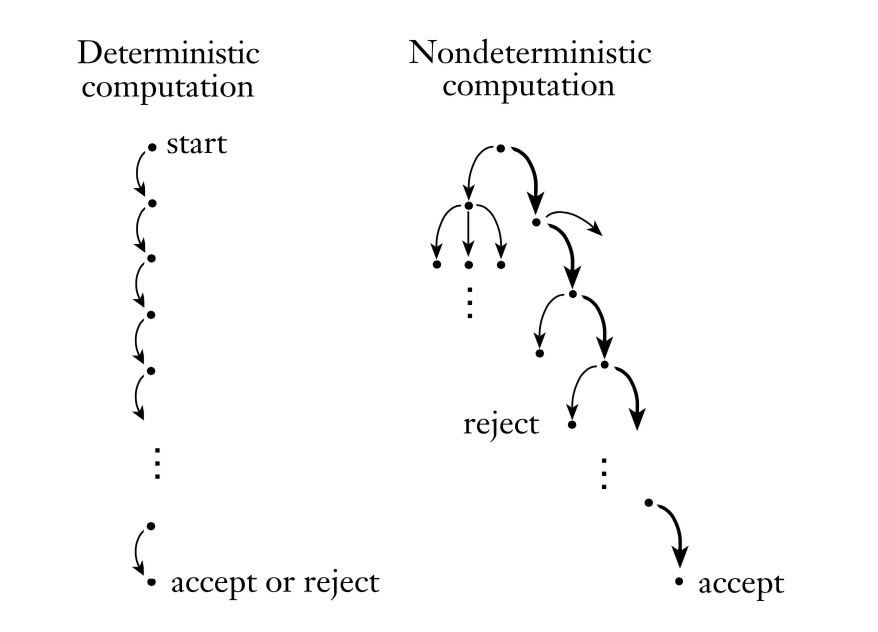
\includegraphics[width=0.5\linewidth]{nfa.png}
    	\caption{Deterministic and nondeterministic computations with an accepting branch}
    	\label{fig}
    \end{figure}
    \item Formal definition of NFA differs from DFA in the type of transition function. In NFA, the transition function takes a state and an input symbol (or empty string), and produces the \textit{set of possible states.}
\end{itemize}
\begin{defn}
A \textbf{\textit{nondeterministic finite automaton}} is a 5-tuple $(Q,\Sigma, \delta, q_0, F)$, where
\begin{enumerate}
    \item $Q$ is a finite set called the states 
    \item $\Sigma$ is a finite alphabet
    \item $\delta: Q\times\Sigma_\epsilon \longrightarrow P(Q)$ is the transition function. Takes a state and an input symbol and produces the set of possible states.
    \item $q_0 \in Q$ is the start state
    \item $F\subseteq Q$ is the set of accept states
\end{enumerate}
\end{defn}

\textbf{\underline{Equivalence of NFAs and DFAs}}
\begin{thm}
Every nondeterministic finite automaton has an equivalent deterministic finite automaton.
\end{thm}
\begin{proof}
    Let $N = (Q, \Sigma, \delta, q_0 , F)$ be the NFA recognizing some language $A$. We construct a DFA $M =(Q',\Sigma,\delta',q_0',F')$ recognizing $A$.Before doing the full construction, let's first consider the easier case wherein $N$ has no $\epsilon$ arrows. Later we take the $\epsilon$ arrows into account.
    \begin{enumerate}
        \item $Q' = P(Q)$\\
        Every state of $M$ is a set of states of $N$.
        \item For $R \in Q'$ and $a \in \Sigma$, let $\delta'(R, a) = \{q \in Q\ |\ q \in \delta(r, a)$ for some $r \in R\}$. If $R$ is a state of $M$, it is also a set of states of $N$. When $M$ reads a symbol $a$ in state $R$, it shows where $a$ takes each state in $R$. Because each state may go to a set of states, we take the union of all these sets. Another way to write this expression is
        \begin{center}
            $\delta'(R,a) = \bigcup_{r\in R} \delta(r,a)$
        \end{center}
        \item $q_0'=\{q_0\}$. $M$ starts in the state corresponding to the collection containing just the start state of $N$.
        \item $F' = \{R\in Q'\ |\ R$ contains an accept state of $N\}$.\\
        The machine M accepts if one of the possible states that N could be in at this point is an accept state.
    \end{enumerate}
    Now we need to consider the $\epsilon$ arrows. To do so, we set up an extra bit of notation.For any state $R$ of $M$, we define $E(R)$ to be the collection of states that can be reached from members of $R$ by going only along $\epsilon$ arrows, including the members of $R$ themselves. Formally, for $R \subseteq Q$ let 
    \begin{center}
        $E(R) = \{q\ |\ q$ can be reached from $R$ by traveling along 0 or more $\epsilon$ arrows$\}$.
    \end{center}
    Then we modify the transition function of $M$ to account for all states that can be reached by going along $\epsilon$ arrows after every step. Replacing $\delta'(r,a)$ by $E(\delta(r, a))$ achieves this effect. Thus
    \begin{center}
        $\delta'(R,a) = \{q\in Q\ |\ q\in E(\delta(r,a))$ for some $r\in R\}$.
    \end{center}
    Additionally, we need to modify the start state of $M$ to account for all possible states that can be reached from the start state of $N$ along the $\epsilon$ arrows. Changing $q_0'$ to be $E(\{q_0\})$ achieves this effect. We have now completed the construction of the DFA $M$ that simulates the NFA $N$.
    The construction of $M$ works correctly. At every step in the computation of $M$ on an input, it clearly enters a state that corresponds to the subset of states that $N$ could be in at that point. Thus our proof is complete.
\end{proof}
\textbf{\underline{Closure under the regular operations}}\\
Using nondeterminism, we can prove that the class of regular languages are closed under the regular operations such as union, cocatenation, and star.
\begin{thm}
The class of regular languages is closed under the union operation.
\end{thm}
\begin{proof}
    \todo{write proof}
\end{proof}
\begin{thm}
The class of regular languages is closed under the concatenation operation.
\end{thm}
\begin{proof}
    \todo{write proof}    
\end{proof}
\begin{thm}
The class of regular languages is closed under the star operation.
\end{thm}
\begin{proof}
        \todo{write proof}
\end{proof}
\subsubsection{Regular expressions}
\begin{defn}
Say that $R$ is a \textbf{\textit{regular expression}} if $R$ is
\begin{enumerate}
    \item $a$ for some $a\in \Sigma$ 
    \item $\epsilon$ 
    \item $\emptyset$
    \item $(R_1\cup R_2$ where $R_1, R_2$ are regular expressions
    \item $(R_1\circ R_2$ where $R_1, R_2$ are regular expressions, or
    \item $(R_1^{*}$ where $R_1$ is a regular expression.
\end{enumerate}
In items 1 and 2, the regular expressions $a$ and $\epsilon$ represent the languages $\{a\}$ and $\{\epsilon\}$, respectively. In item 3, the regular expression $\emptyset$ represents the empty language. In items 4, 5, and 6, the expressions represent the languages obtained by taking the union or concatenation of the languages $R_1$ and $R_2$, or the star of the language $R_1$, respectively.
\end{defn}
\textbf{\underline{Equivalence with finite automata}}
\begin{thm}
A language is regular iff some regular expression describes it.
\end{thm}

\todo{finish the proof for this part }
\begin{lemma}
    If a language is described by a regular expression, then it is regular.
\end{lemma}
 
\begin{proof}

\end{proof}
\begin{lemma}
If a language is regular, then it is described by a regular expression.
\end{lemma}
\begin{defn}
A \textbf{\textit{generalized nondeterministic finite automaton}} (GNFA) is a 5-tuple $(Q,\Sigma, \delta, q_{start}, q_{accept})$, where
\begin{enumerate}
    \item $Q$ is a finite set called the states 
    \item $\Sigma$ is the input alphabet
    \item $\delta: (Q-\{q_{accept}\})\times(Q-\{q_{start}\}) \longrightarrow R$ is the transition function, where $R$ is the collection of all regular expressions over the alphabet $\Sigma$
    \item $q_{start}$ is the start state
    \item $q_{accept}$ is the accept state
\end{enumerate}
\end{defn}

\subsubsection{Nonregular languages}
\textbf{\underline{The pumping lemma for regular languages}}
\begin{thm}
    If $A$ is a regular language, then there is a number $p$ (the pumping length) where if $s$ is any string in $A$ of length at least $p$, then $s$ may be divided into three pieces, $s = xyz$, satisfying the following conditions:
    \begin{enumerate}
        \item for each $i\geq 0, xy^iz\in A$,
        \item $|y|>0$, and
        \item $|xy| \leq p$.
    \end{enumerate}
When $s$ is divided into $xyz$, either $x$ or $z$ may be $\epsilon$, but condition 2 says that $y \neq \epsilon$. $x$ and $y$ together have length at most $p$.
\end{thm}

\subsection{Context-free languages}
\subsubsection{Context-free grammars}
\begin{itemize}[leftmargin=*]
    \item A grammar consists of a collection of \textbf{substitution rules}, aka \textbf{productions}.
\end{itemize}
\begin{defn}
A \textbf{\textit{context-free grammar}} is a 4-tuple $(V,\Sigma,R,S)$, where
\begin{enumerate}
    \item $V$ is a finite set called the variables,
    \item $\Sigma$ is a finite set, disjoint from $V$, called the terminals,
    \item $R$ is a finite set of rules, with each rule being a variable and a string of variables and terminals, and
    \item $S\in V$ is the start variable
\end{enumerate}
The language of the grammar is $\{w \in \Sigma^{^{*}}\ |\ S \Rightarrow^{^{*}} w\}$.
\end{defn}
\begin{defn}
A string $w$ is derived ambiguously in context-free grammar $G$ if it has two or more different leftmost derivations. Grammar $G$ is ambiguous if it generates some string ambiguously.
\end{defn}
\textbf{\underline{Chomsky Normal Form}}
\begin{defn}
A context-free grammar is in \textbf{Chomsky normal form} if every rule is
of the form
    \begin{center}
        $A \to BC$\\
        $A \to a$
    \end{center}
where $a$ is any terminal and $A, B,$ and $C$ are any variables, except that $B$ and $C$ may not be the start variable. In addition, we permit the rule $S\to \epsilon$, where $S$ is the start variable.
\end{defn}
\begin{itemize}[leftmargin=*]
    \item For any string $w\in L(G)$ of length $n\geq 1$, exactly $2n-1$ steps are required for the derivation of $w$, if $G$ is in Chomsky Normal Form (CNF)
\end{itemize}
\begin{thm}
    Any context-free language is generated by a context-free grammar in Chomsky
normal form.
\end{thm}
\begin{proof}
We can convert any grammar $G$ into CNF: (p.109)
\begin{enumerate}
    \item Add a new start variable $S_0\to S$
    \item Eliminate all $\epsilon$-rules: remove an $\epsilon$-rule $A\to \epsilon$
    \item Eliminate all unit-rules. We remove a unit rule $A \to B$. Then, whenever a rule $B \to u$ appears, we add the rule $A \to u$ unless this was a unit rule previously removed. As before, $u$ is a string of variables and terminals. We repeat these steps until we eliminate all unit rules.
    \item Convert all remaining rules into proper form.
\end{enumerate}
\end{proof}
\subsubsection{Pushdown automata}
\begin{itemize}[leftmargin=*]
    \item Pushdown automata are equivalent in power to context-free grammars.
    \item A schematic representation of a pushdown automaton. The control represents the states and transition function, the tape contains the input string, and the arrow represents the input head, pointing at the next input symbol to be read. The pushdown automaton has a stack component.
    \begin{figure}[h]
    	\centering
    	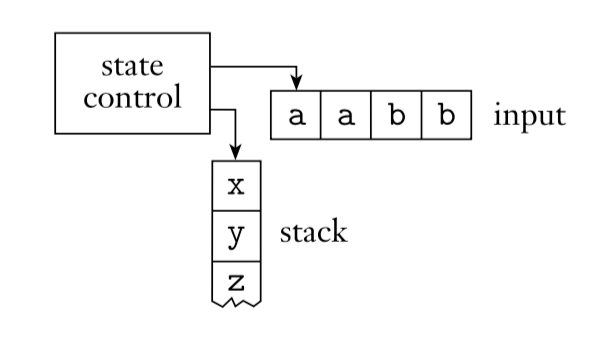
\includegraphics[width=0.5\linewidth]{pda.png}
    	\caption{Schematic of a pushdown automaton}
    	\label{fig}
    \end{figure}
    \item Pushing a symbol: Writing a symbol on the stack tape
    \item Popping a symbol: Removing a symbol from the stack tape 
\end{itemize}
\begin{defn}
A \textbf{\textit{pushdown automaton}} is a 6-tuple $(Q,\Sigma, \Gamma, \delta, q_0, F)$, where $Q,\Sigma, \Gamma,  F$ are all finite sets, and
\begin{enumerate}
    \item $Q$ is the set of states
    \item $\Sigma$ is the input alphabet
    \item $\Gamma$ is the stack alphabet
    \item $\delta:Q\times\Sigma_\epsilon\times \Gamma_\epsilon\to \wp(Q\times\Gamma_\epsilon$ is the transition function
    \item $q_0\in Q$ is the start state, and 
    \item $F\subseteq Q$ is the set of accept states.
\end{enumerate}
A pushdown automaton $M = (Q,\Sigma, \Gamma, \delta, q_0, F)$ computes as follows: It accepts input $w$ if $w$ can be written as $w=w_1w_2\ldots w_m$, where each $w_i\in \Sigma_\epsilon$ and sequences of states $r_0,r_1,\ldots, r_m\in Q$ and strings $s_0,s_1,\ldots,s_m\in \Gamma^*$ exist that satisfy the following conditions. The strings $s_i$ represent the sequence of stack contents that $M$ has on the accepting branch of the computation.
\begin{enumerate}
    \item $r_0 = q_0$ and $s_0 = \epsilon$. $M$ starts out properly, in the start state and with an empty stack.
    \item For $i=0,\ldots, m-1$, we have $(r_{i+1}, b)\in \delta(r_i, w_{i+1}, a)$, where $s_i = at$ and $s_{i+1} = bt$ for some $a,b\in \Gamma_\epsilon$ and $t\in\Gamma^*$. $M$ moves properly according to the state, stack, and next input symbol.
    \item $r_m\in F$. An accept state occurs at the input end.
\end{enumerate}
\end{defn}
\textbf{\underline{Equivalence with context-free grammars}}
\begin{thm}
    A language is context-free iff some pushdown automaton recognizes it.
\end{thm}
\begin{lemma}
If a language is context free, then some pushdown automaton recognizes it.
\end{lemma}
\begin{lemma}
If a pushdown automaton recognizes some language, then it is context free.
\end{lemma}
\subsubsection{Non-context-free languages}
\textbf{\underline{The pumping lemma for context-free languages}}
\begin{thm}
    If $A$ is a context-free language, then there is a number $p$ (the pumping length) where if $s$ is any string in $A$ of length at least $p$, then $s$ may be divided into five pieces, $s = uvxyz$, satisfying the following conditions:
    \begin{enumerate}
        \item for each $i\geq 0, uv^ixy^iz\in A$,
        \item $|vy|>0$, and
        \item $|vxy| \leq p$.
    \end{enumerate}
When $s$ is divided into $xyz$, either $x$ or $z$ may be $\epsilon$, but condition 2 says that $y \neq \epsilon$. $x$ and $y$ together have length at most $p$.
\end{thm}
\pagebreak
\section{Computability Theory}
\subsection{Turing machines}
\begin{itemize}[leftmargin=*]
    \item Turing machines use an infinite tape as its unlimited memory.
    \item It has a tape head that can read and write symbols and move around on the tape.
    \item The schematic of a Turing Machine:
    \begin{figure}[h]
    	\centering
    	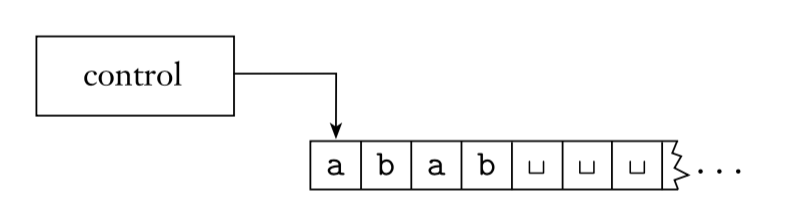
\includegraphics[width=0.5\linewidth]{tm.png}
    	\caption{Schematic of a Turing machine}
    	\label{fig}
    \end{figure}
    \item The collection of strings that a Turing machine $M$ accepts is the language or $M$, or the language recognized by $M$, denoted by $L(M)$.
\end{itemize}
\textbf{\underline{Differences between finite automata and Turing machines}}
\begin{enumerate}
    \item A Turing machine can both write on the tape and read from it.
    \item The read–write head can move both to the left and to the right.
    \item The tape is infinite.
    \item The special states for rejecting and accepting take effect immediately.
\end{enumerate}
\begin{defn}
A \textbf{\textit{Turing machine}} is a 7-tuple $(Q,\Sigma, \Gamma, \delta, q_0, q_{accept},q_{reject})$, where $Q,\Sigma, \Gamma$ are all finite sets, and
\begin{enumerate}
    \item $Q$ is the set of states
    \item $\Sigma$ is the input alphabet not containing the blank symbol $\sqcup$,
    \item $\Gamma$ is the tape alphabet, where $\sqcup\in\Gamma$ and $\Sigma\subseteq\Gamma$,
    \item $\delta:Q\times\Gamma\to Q\times\Gamma\times \{L,R\}$ is the transition function
    \item $q_0\in Q$ is the start state, 
    \item $q_{accept}\in Q$ is the accept state, and 
    \item $q_{reject}\in Q$ is the reject state.
\end{enumerate}
A Turing machine $M = (Q,\Sigma, \Gamma, \delta, q_0, q_{accept},q_{reject})$ computes as follows. Initially, $M$ receives its input $w = w_1w_2\ldots w_n \in\Sigma^*$ on the leftmost $n$ squares of the tape, and the rest of the tape is blank (i.e., filled with blank symbols). The head starts on the leftmost square of the tape. Note that $\Sigma$ does not contain the blank symbol, so the first blank appearing on the tape marks the end of the input. Once $M$ has started, the computation proceeds according to the rules described by the transition function. If $M$ ever tries to move its head to the left off the left-hand end of the tape, the head stays in the same place for that move, even though the transition function indicates L. The computation continues until it enters either the accept or reject states, at which point it halts. If neither occurs, $M$ goes on forever.\\\\
As a Turing machine computes, changes occur in the current state, the current tape contents, and the current head location. A setting of these three items is called a configuration of the Turing machine. Configurations often are represented in a special way. For a state $q$ and two strings $u$ and $v$ over the tape alphabet $\Gamma$, we write $u q v$ for the configuration where the current state is $q$, the current tape contents is $uv$, and the current head location is the first symbol of $v$. The tape contains only blanks following the last symbol of $v$. 
\end{defn}
\begin{defn}
Call a language Turing-recognizable if some Turing machine recognizes it.
\end{defn}
\begin{defn}
Call a language Turing-decidable or simply decidable if some Turing machine decides it.\\\\
A Turing machines that halt on all inputs, never loops. These machines are called deciders because they always make a decision to accept or reject. A decider that recognizes some language also is said to decide that language.
\end{defn}
\subsection{Variants of Turing machines}
\begin{itemize}[leftmargin=*]
    \item Variants of TMs and the original TM all have the same power because they recognize the same class of languages.
    \item Robustness: invariance to certain changes in the definition.
\end{itemize}
\textbf{\underline{Multitape Turing machine}}
\begin{thm}
    Every multitape Turing machine has an equivalent single-tape Turing machine.
\end{thm}
\begin{thm}
    A language is Turing-recognizable if and only if some multitape Turing machine recognizes it.
\end{thm}
\textbf{\underline{Nondeterministic Turing machine}}
\begin{itemize}[leftmargin=*]
    \item The transition function for a nondeterministic Turing machine has the form
    \begin{center}
        $\delta:Q\times\Gamma\to\wp(Q\times\Gamma\times\{L,R\})$
    \end{center}
    \item The computation of a nondeterministic Turing machine is a tree whose branches correspond to different possibilities for the machine. 
    \item If some branch of the computation leads to the accept state, the machine accepts its input.
\end{itemize}
\begin{thm}
    Every nondeterministic Turing machine has an equivalent deterministic Turing machine.
\end{thm}
\begin{thm}
    A language is Turing-recognizable if and only if some nondeterministic Turing machine recognizes it.
\end{thm}
\begin{thm}
    A language is decidable if and only if some nondeterministic Turing machine
decides it.
\end{thm}
\textbf{\underline{Enumerators}}
\begin{itemize}[leftmargin=*]
    \item Turing-recognizable languages = recursively enumerable language
    \item An enumerator is a Turing machine with an attached printer
    \item The Turing machine can use that printer as an output device to print strings. 
    \item Every time the Turing machine wants to add a string to the list, it sends the string to the printer.
    \item An enumerator $E$ starts with a blank input on its work tape. If the enumerator doesn't halt, it may print an infinite list of strings. The language enumerated by $E$ is the collection of all the strings that it eventually prints out. Moreover, $E$ may generate the strings of the language in any order, possibly with repetitions.
\end{itemize}
\begin{thm}
    A language is Turing-recognizable if and only if some enumerator enumerates it.
\end{thm}
\todo{proofs and equivalence phenomenon}

% \subsection{Algorithm definition}
% \begin{itemize}[leftmargin=*]
%     \item An algorithm is a collection of simple instructions for carrying out some task
% \end{itemize}

\subsection{Decidability}
\begin{itemize}[leftmargin=*]
    \item Certain problems can be solved algorithmically and others cannot -- exploring the limits of algorithmic solvability
\end{itemize}
\subsubsection{Decidable problems concerning regular languages}
\begin{thm}
    $A_{DFA}$ is a decidable language.
    \begin{center}
        $A_{DFA} = \{\langle B,w\rangle\ |\ B$ is a DFA that accepts input string $w\}$.
    \end{center}
    The problem of testing whether a DFA $B$ accepts an input $w$ is the same as the problem of testing whether $\langle B, w\rangle$ is a member of the language $A_{DFA}$. Similarly, we can formulate other computational problems in terms of testing membership in a language. Showing that the language is decidable is the same as showing that the computational problem is decidable.
\end{thm}
\begin{proof}
    \todo{proofs for this section}
\end{proof}
\begin{thm}
    $A_{NFA}$ is a decidable language.
    \begin{center}
        $A_{NFA} = \{\langle B,w\rangle\ |\ B$ is a NFA that accepts input string $w\}$.
    \end{center}
\end{thm}
\begin{proof}
    \todo{proofs for this section}
\end{proof}
\begin{thm}
    $A_{REX}$ is a decidable language.
    \begin{center}
        $A_{REX} = \{\langle R,w\rangle\ |\ R$ is a regular expression that generates string $w\}$.
    \end{center}
\end{thm}
\begin{proof}
    \todo{proofs for this section}
\end{proof}
\begin{thm}
    $E_{DFA}$ is a decidable language.
    \begin{center}
        $E_{DFA} = \{\langle A\rangle\ |\ A$ is a DFA and $L(A)=\emptyset\}$.
    \end{center}
\end{thm}
\begin{proof}
    \todo{proofs for this section}
\end{proof}
\begin{thm}
    $EQ_{DFA}$ is a decidable language.
    \begin{center}
        $EQ_{DFA} =\{\langle A, B\rangle\ |\ A$ and $B$ are DFAs and $L(A)=L(B)\}$.
    \end{center}
\end{thm}
\begin{proof}
    \todo{proofs for this section}
\end{proof}

\subsubsection{Decidable problems concerning context-free languages}
\begin{thm}
    $A_{CFG}$ is a decidable language.
    \begin{center}
        $A_{CFG} = \{\langle G,w\rangle\ |\ G$ is a CFG that generates string $w\}$.
    \end{center}
\end{thm}
\begin{proof}
    \todo{proofs for this section}
\end{proof}
\begin{thm}
    $E_{CFG}$ is a decidable language.
    \begin{center}
        $E_{CFG} = \{\langle G\rangle\ |\ G$ is a CFG and $L(G)=\emptyset\}$.
    \end{center}
\end{thm}
\begin{proof}
    \todo{proofs for this section}
\end{proof}
\begin{thm}
    Every context-free language is decidable.
\end{thm}
\begin{proof}
    \todo{proofs for this section}
\end{proof}
\subsection{Undecidability}
\subsection{Undecidable problems from language theory}
\subsection{Mapping reducibility}

\section{Complexity Theory}
\subsection{Measuring complexity}
\subsection{The class P}
\subsection{The class NP}
\subsection{NP-Completeness}


\end{document}